\appendix
\section{Appendix}

\begin{frame}{Analyze virtualized machine}
\code{perf} has support for the Kernel-based Virtual Machine (KVM \cite{kvm}). For the performance measurement, an argument tells \code{perf} that the machine using KVM should be monitored. It uses the PMU of the host. It seems that also detailed information is available if the host machine has access to the guests \code{/proc/} files. Measures of hardware counters from inside the virtual machine is not supported.

VirtualBox \cite{virtualbox} is not supported. This has two consequences. First, \code{perf} on the host can not record data about the guest. Second, there is no PMU in the virtual machine and therefore \code{perf} can not record hardware counters.
\end{frame}

\begin{frame}{detailed file format\label{sec:fileformat}}
\centering{
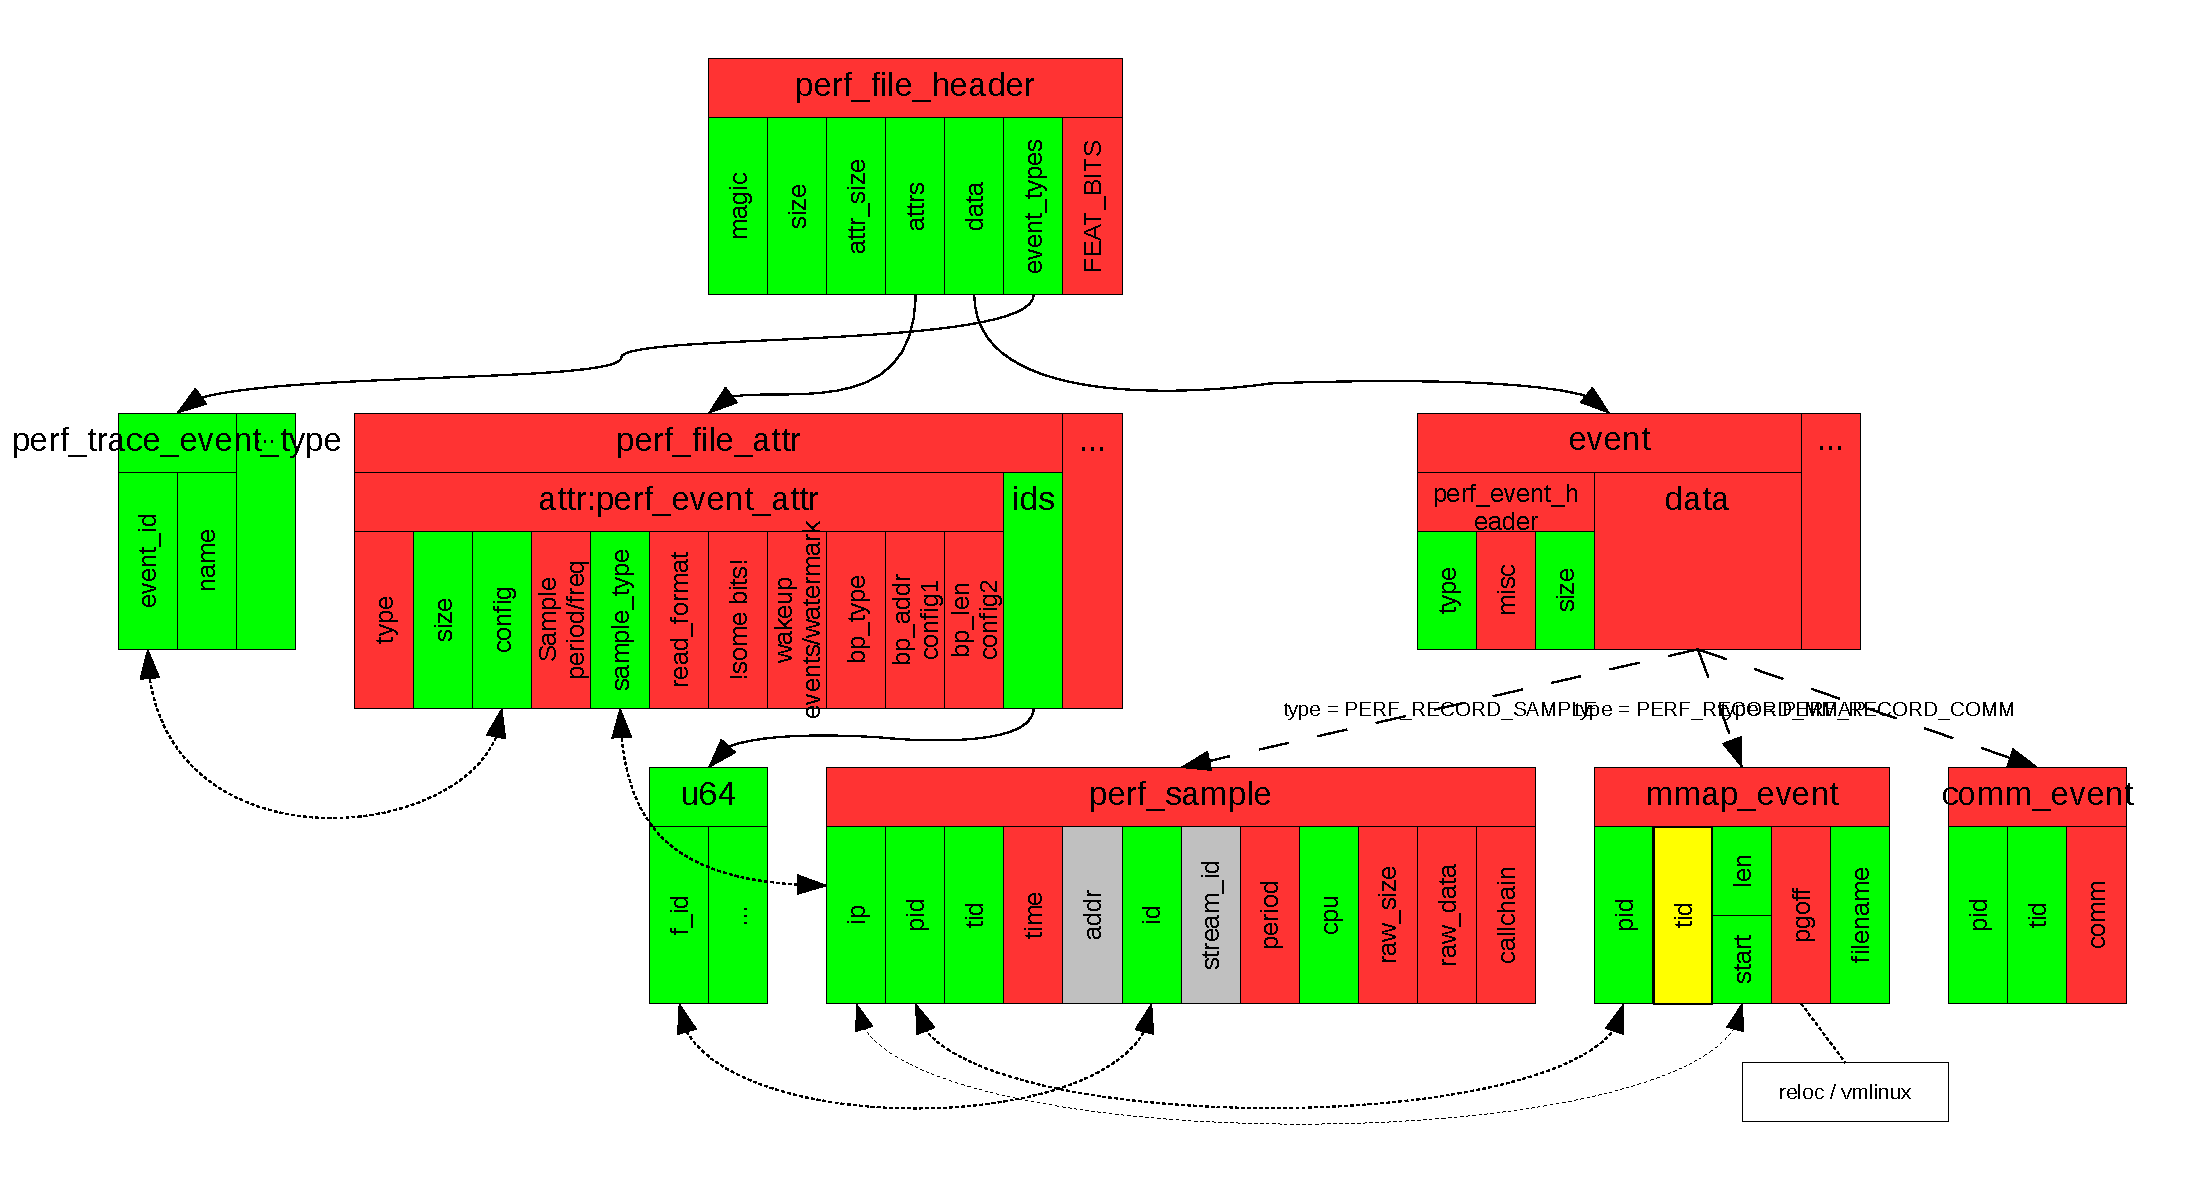
\includegraphics[width=12cm]{res/fileformat}
}
\end{frame}

\only<handout>{
\begin{frame}{literature}
\begin{scriptsize}
  \printbibliography
\end{scriptsize}
\end{frame}
}
